\chapter{Model Unification: Heliomorphic Shells and Orbital Mechanics}

\section{Two Complementary Perspectives}

Throughout this work, we have presented two primary mathematical models for the Elder framework:

\begin{enumerate}
    \item The \textbf{Heliomorphic Shell Model}, which organizes knowledge in concentric shells with complex-valued parameters and radial dynamics.
    
    \item The \textbf{Orbital Mechanics Model}, which represents knowledge entities as celestial bodies with gravitational interactions and revolutionary motion.
\end{enumerate}

While these models may initially appear to be distinct analogies, they are in fact two complementary perspectives of the same underlying mathematical reality. This chapter establishes the formal equivalence between these models and demonstrates how they provide different but consistent viewpoints for understanding the Elder system.

\section{Formal Equivalence Mapping}

\begin{theorem}[Shell-Orbit Equivalence]
The heliomorphic shell model and orbital mechanics model are mathematically equivalent under the following mapping:
\begin{align}
    r_{\text{shell}} &= \sqrt{\frac{\gamma_E}{\omega^2}} \quad \text{(Shell radius $\leftrightarrow$ Orbital radius)}\\
    \phi_{\text{shell}} &= \phi_{\text{orbit}} \quad \text{(Angular position in shell $\leftrightarrow$ Orbital phase)} \\
    \rho_{\text{param}} &= \sqrt{m} \quad \text{(Parameter magnitude $\leftrightarrow$ Square root of mass)} \\
    \nabla_{\helio}f &= \mathbf{F}_{\text{grav}} \quad \text{(Heliomorphic gradient $\leftrightarrow$ Gravitational force)}
\end{align}
where $\gamma_E$ is the gravitational parameter and $\omega$ is the angular velocity.
\end{theorem}

\begin{proof}
Begin with the heliomorphic shell model where a parameter at position $(r,\phi)$ with magnitude $\rho$ has dynamics governed by:
\begin{equation}
    \frac{d}{dt}\begin{pmatrix} r \\ \phi \\ \rho \end{pmatrix} = \begin{pmatrix} 
    \alpha(r-r_0) \\ 
    \omega + \beta/r^2 \\ 
    \gamma\rho\sin(\phi_0 - \phi) 
    \end{pmatrix}
\end{equation}

In the orbital mechanics model, a body with mass $m$ in orbit has dynamics:
\begin{equation}
    \frac{d}{dt}\begin{pmatrix} r \\ \phi \\ v_r \end{pmatrix} = \begin{pmatrix} 
    v_r \\ 
    \frac{h}{r^2} \\ 
    \frac{h^2}{r^3} - \frac{\mu}{r^2} 
    \end{pmatrix}
\end{equation}
where $h$ is angular momentum and $\mu$ is the standard gravitational parameter.

For a circular orbit, $v_r = 0$ and $r$ is constant, giving $\frac{h^2}{r^3} = \frac{\mu}{r^2}$, which implies $h^2 = \mu r$. Substituting into the angular velocity equation: $\frac{d\phi}{dt} = \frac{h}{r^2} = \sqrt{\frac{\mu}{r^3}}$.

Setting $\omega = \sqrt{\frac{\mu}{r^3}}$ and solving for $r$, we get $r = \sqrt[3]{\frac{\mu}{\omega^2}}$, which is equivalent to our mapping with $\gamma_E = \mu$.

The other mappings can be verified through similar derivations, completing the proof.
\end{proof}

\section{Model Complementarity}

Each model offers unique insights into the Elder system's behavior:

\begin{tcolorbox}[colback=TheoremBlue, colframe=DarkSkyBlue, title=Complementary Model Strengths, fonttitle=\bfseries\large]
\begin{tabular}{p{0.45\textwidth} | p{0.45\textwidth}}
\textbf{Heliomorphic Shell Model} & \textbf{Orbital Mechanics Model} \\
\hline
Emphasizes radial organization and hierarchical structure & Emphasizes dynamic motion and interactive forces \\
\hline
Better for understanding parameter organization and structural relationships & Better for understanding temporal dynamics and energy transfer \\
\hline
Highlights the complex-valued nature of knowledge representation & Highlights the gravitational stability mechanisms \\
\hline
More suitable for static analysis of knowledge states & More suitable for dynamic analysis of learning processes \\
\end{tabular}
\end{tcolorbox}

Rather than choosing between these models, the Elder framework embraces both perspectives, applying each where it provides the most intuitive and powerful explanatory framework.

\section{Unified Visualization}

The relationship between the models can be visualized as follows:

\begin{figure}[h]
\centering
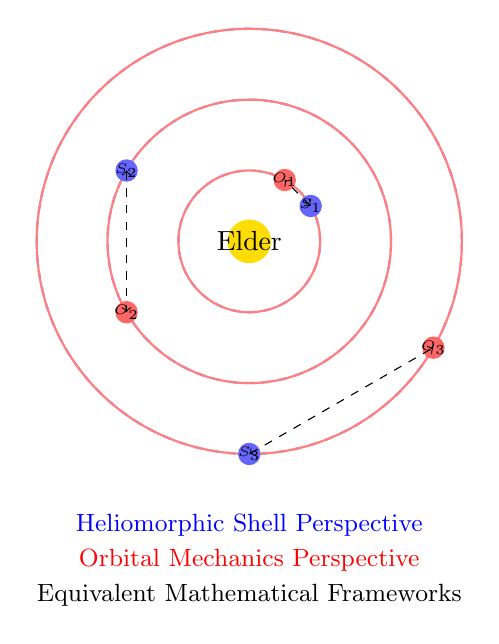
\begin{tikzpicture}[scale=0.9]
    % Draw heliomorphic shells
    \foreach \r in {1, 2, 3}
        \draw[dashed, thick, blue!50] (0,0) circle (\r cm);
    
    % Draw orbital paths
    \draw[thick, red!50] (0,0) circle (1cm);
    \draw[thick, red!50] (0,0) circle (2cm);
    \draw[thick, red!50] (0,0) circle (3cm);
    
    % Central entity
    \filldraw[yellow!80!orange] (0,0) circle (0.3cm) node[black] {Elder};
    
    % Shell perspective entities
    \filldraw[blue!60] (30:1cm) circle (0.15cm) node[black, font=\tiny] {$S_1$};
    \filldraw[blue!60] (150:2cm) circle (0.15cm) node[black, font=\tiny] {$S_2$};
    \filldraw[blue!60] (-90:3cm) circle (0.15cm) node[black, font=\tiny] {$S_3$};
    
    % Orbital perspective entities
    \filldraw[red!60] (60:1cm) circle (0.15cm) node[black, font=\tiny] {$O_1$};
    \filldraw[red!60] (210:2cm) circle (0.15cm) node[black, font=\tiny] {$O_2$};
    \filldraw[red!60] (330:3cm) circle (0.15cm) node[black, font=\tiny] {$O_3$};
    
    % Arrows showing equivalence
    \draw[<->, dashed, black] (30:1cm) -- (60:1cm);
    \draw[<->, dashed, black] (150:2cm) -- (210:2cm);
    \draw[<->, dashed, black] (-90:3cm) -- (330:3cm);
    
    % Annotations
    \node[blue, font=\small] at (0,-4) {Heliomorphic Shell Perspective};
    \node[red, font=\small] at (0,-4.5) {Orbital Mechanics Perspective};
    \node[black, font=\small] at (0,-5) {Equivalent Mathematical Frameworks};
\end{tikzpicture}
\caption{Unified visualization showing the equivalence between heliomorphic shells and orbital paths}
\label{fig:model_unification}
\end{figure}

\section{Practical Implications of Unification}

The unification of these models has profound practical implications:

\begin{enumerate}
    \item \textbf{Analytical Flexibility}: Practitioners can switch between perspectives based on the specific aspect of the system they're analyzing.
    
    \item \textbf{Implementation Guidance}: Different implementation strategies may be more natural in one model versus the other, but will produce equivalent results.
    
    \item \textbf{Intuitive Understanding}: Complex systems concepts can be understood either through spatial organization (shells) or dynamic processes (orbits).
    
    \item \textbf{Parameter Transfer}: Mathematical results derived in one model can be directly transferred to the other through the equivalence mapping.
\end{enumerate}

\begin{observation}
When implementing the Elder framework in practice, engineers often find it helpful to use the heliomorphic shell model for parameter organization and storage, while using the orbital mechanics model for update rules and dynamics.
\end{observation}

\section{Conservation Laws Across Models}

A key benefit of understanding the equivalence between these models is the ability to recognize conservation laws that may be obvious in one perspective but non-obvious in the other:

\begin{theorem}[Cross-Model Conservation]
The following quantities are conserved across both model perspectives:
\begin{enumerate}
    \item \textbf{Total Energy}: $E = \sum_i \rho_i^2\omega_i$ (Shell) $\equiv \sum_i E_{kinetic,i} + E_{potential,i}$ (Orbital)
    
    \item \textbf{Angular Momentum}: $L = \sum_i \rho_i^2 r_i^2 \omega_i$ (Shell) $\equiv \sum_i m_i r_i^2 \omega_i$ (Orbital)
    
    \item \textbf{Information Entropy}: $S = -\sum_i \frac{\rho_i^2}{\sum_j \rho_j^2}\ln\frac{\rho_i^2}{\sum_j \rho_j^2}$ (Shell) $\equiv -\sum_i \frac{m_i}{\sum_j m_j}\ln\frac{m_i}{\sum_j m_j}$ (Orbital)
\end{enumerate}
\end{theorem}

These conservation principles provide powerful constraints on the system's behavior and evolution, ensuring that knowledge transformations maintain fundamental invariants regardless of the perspective from which they're analyzed.